\documentclass[a4paper,11pt]{article}
\input{/home/tof/Documents/Cozy/latex-include/preambule_lua.tex}
\newcommand{\showprof}{show them}  % comment this line if you don't want to see todo environment
\fancyhead[L]{Liste chaînée}
\newdate{madate}{10}{09}{2020}
\fancyhead[R]{Terminale - NSI} %\today
\fancyfoot[L]{~\\Christophe Viroulaud}
\fancyfoot[C]{\textbf{Page \thepage}}
\fancyfoot[R]{\includegraphics[width=2cm,align=t]{/home/tof/Documents/Cozy/latex-include/cc.png}}
\usepackage{tikz}

\begin{document}
\begin{Form}
\begin{commentprof}
Problématique étendue sur ce chapitre et le suivant( pile,file): représenter la liste des processus dans l'ordonnanceur.
\end{commentprof}
\section{Problématique}
Quand nous créons un tableau, un espace fixé par la taille du tableau est alloué en mémoire. 
\begin{figure}[!h]
\centering
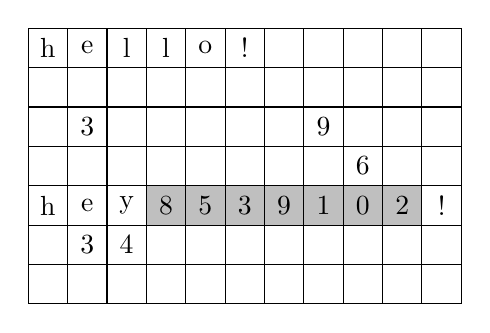
\begin{tikzpicture}[scale=0.5]
\fill[gray!50] (3,2) rectangle (10,3);
\draw (0,0) grid (11,7);

\draw (0.5,2.5) node{h};
\draw (1.5,2.5) node{e};
\draw (2.5,2.5) node{y};

\draw (0.5,6.5) node{h};
\draw (1.5,6.5) node{e};
\draw (2.5,6.5) node{l};
\draw (3.5,6.5) node{l};
\draw (4.5,6.5) node{o};
\draw (5.5,6.5) node{!};

\draw (10.5,2.5) node{!};
\draw (7.5,4.5) node{9};
\draw (8.5,3.5) node{6};
\draw (1.5,4.5) node{3};
\draw (2.5,1.5) node{4};
\draw (1.5,1.5) node{3};

\foreach \x/\y in {3/8,4/5,5/3,6/9,7/1,8/0,9/2}
{\draw (\x+0.5,2.5) node{\y};}
\end{tikzpicture}
\captionof{figure}{Le tableau est enregistré dans un espace libre}
\end{figure}
\\Ce comportement permet d'accéder \textit{en temps constant} à chaque élément du tableau. Cependant insérer un nouvel élément devient problématique: il faut trouver un nouvel espace libre et recopier entièrement le tableau augmenté de la nouvelle valeur.
\begin{center}
\shadowbox{\parbox{15cm}{\centering Peut-on définir un autre type de structure pour représenter les données en mémoire?}}
\end{center}
\section{Liste chaînée}
\subsection{Principe}
Chaque élément est stocké dans un espace de la mémoire. De plus chaque maillon de la chaîne possède une seconde information: l'adresse du maillon suivant.
\begin{figure}[!h]
\centering
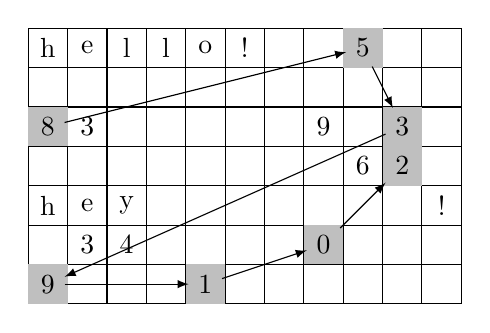
\begin{tikzpicture}[scale=0.5]
\draw (0,0) grid (11,7);

\draw (0.5,2.5) node{h};
\draw (1.5,2.5) node{e};
\draw (2.5,2.5) node{y};

\draw (0.5,6.5) node{h};
\draw (1.5,6.5) node{e};
\draw (2.5,6.5) node{l};
\draw (3.5,6.5) node{l};
\draw (4.5,6.5) node{o};
\draw (5.5,6.5) node{!};

\draw (10.5,2.5) node{!};
\draw (7.5,4.5) node{9};
\draw (8.5,3.5) node{6};
\draw (1.5,4.5) node{3};
\draw (2.5,1.5) node{4};
\draw (1.5,1.5) node{3};

\fill[gray!50] (0,4) rectangle (1,5);
\node (8) at (0.5,4.5) {8};
\fill[gray!50] (8,6) rectangle (9,7);
\node (5) at (8.5,6.5) {5};
\fill[gray!50] (9,4) rectangle (10,5);
\node (3) at (9.5,4.5) {3};
\fill[gray!50] (0,0) rectangle (1,1);
\node (9) at (0.5,0.5) {9};
\fill[gray!50] (4,0) rectangle (5,1);
\node (1) at (4.5,0.5) {1};
\fill[gray!50] (7,1) rectangle (8,2);
\node (0) at (7.5,1.5) {0};
\fill[gray!50] (9,3) rectangle (10,4);
\node (2) at (9.5,3.5) {2};
\draw[->,>=latex] (8) -- (5);
\draw[->,>=latex] (5) -- (3);
\draw[->,>=latex] (3) -- (9);
\draw[->,>=latex] (9) -- (1);
\draw[->,>=latex] (1) -- (0);
\draw[->,>=latex] (0) -- (2);
\end{tikzpicture}
\captionof{figure}{Chaque élément occupe un espace libre}
\end{figure}

Nous travaillerons sur des listes contenant des entiers.
\subsection{Le maillon}
Créons un objet \textit{Maillon} qui contiendra la valeur de l'élément et un pointeur vers le maillon suivant.
\lstinputlisting[firstline=10,lastline=16]{"scripts/liste.py"}
\subsection{La liste}
Pour construire une liste il suffit de créer des instances de ce \textit{Maillon}:
\begin{lstlisting}
lst = Maillon(3, Maillon(5, Maillon(8, None)))
\end{lstlisting}
La liste pointe sur le dernier élément ajouté. Le premier élément n'a pas de \textit{suivant}.
\begin{figure}[!h]
\centering
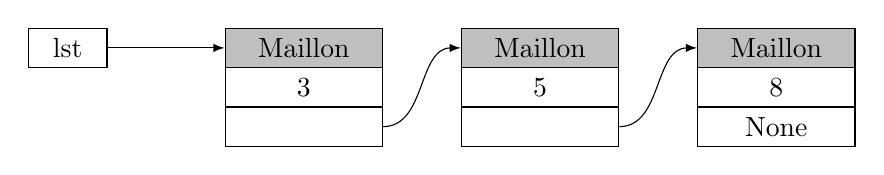
\begin{tikzpicture}[scale=0.5]
\node[draw,minimum width=1cm, minimum height=0.5cm] (lst) at (-6,2) {lst};

\node[draw,fill=gray!50,minimum width=2cm, minimum height=0.5cm] (c10) at (0,2) {Maillon};
\node[draw,minimum width=2cm, minimum height=0.5cm] (c11) at (0,1) {3};
\node[draw,minimum width=2cm, minimum height=0.5cm] (c12) at (0,0) {};

\node[draw,fill=gray!50,minimum width=2cm, minimum height=0.5cm] (c20) at (6,2) {Maillon};
\node[draw,minimum width=2cm, minimum height=0.5cm] (c21) at (6,1) {5};
\node[draw,minimum width=2cm, minimum height=0.5cm] (c22) at (6,0) {};

\node[draw,fill=gray!50,minimum width=2cm, minimum height=0.5cm] (c30) at (12,2) {Maillon};
\node[draw,minimum width=2cm, minimum height=0.5cm] (c31) at (12,1) {8};
\node[draw,minimum width=2cm, minimum height=0.5cm] (c32) at (12,0) {None};

\draw[->,>=latex] (lst) -- (c10);
\draw[->,>=latex] (c12) to[out=0,in=180] (c20);
\draw[->,>=latex] (c22) to[out=0,in=180] (c30);
\end{tikzpicture}
\captionof{figure}{La liste est une succession de maillons}
\end{figure}
\\Une seconde approche consiste en la création d'une classe \textit{liste}.
\lstinputlisting[firstline=18,lastline=23]{"scripts/liste.py"}	
\begin{figure}[!h]
\centering
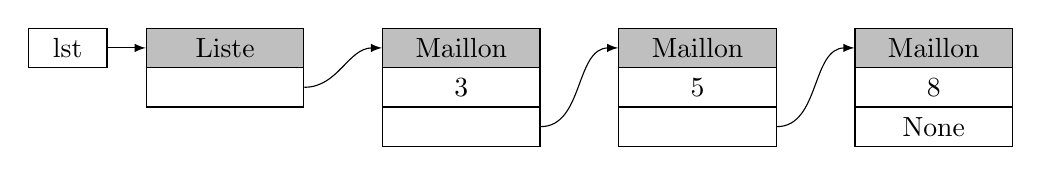
\begin{tikzpicture}[scale=0.5]
\node[draw,minimum width=1cm, minimum height=0.5cm] (lst) at (-10,2) {lst};

\node[draw,fill=gray!50,minimum width=2cm, minimum height=0.5cm] (liste) at (-6,2) {Liste};
\node[draw,minimum width=2cm, minimum height=0.5cm] (l) at (-6,1) {};

\node[draw,fill=gray!50,minimum width=2cm, minimum height=0.5cm] (c10) at (0,2) {Maillon};
\node[draw,minimum width=2cm, minimum height=0.5cm] (c11) at (0,1) {3};
\node[draw,minimum width=2cm, minimum height=0.5cm] (c12) at (0,0) {};

\node[draw,fill=gray!50,minimum width=2cm, minimum height=0.5cm] (c20) at (6,2) {Maillon};
\node[draw,minimum width=2cm, minimum height=0.5cm] (c21) at (6,1) {5};
\node[draw,minimum width=2cm, minimum height=0.5cm] (c22) at (6,0) {};

\node[draw,fill=gray!50,minimum width=2cm, minimum height=0.5cm] (c30) at (12,2) {Maillon};
\node[draw,minimum width=2cm, minimum height=0.5cm] (c31) at (12,1) {8};
\node[draw,minimum width=2cm, minimum height=0.5cm] (c32) at (12,0) {None};

\draw[->,>=latex] (lst) -- (liste);
\draw[->,>=latex] (l) to[out=0,in=180] (c10);
\draw[->,>=latex] (c12) to[out=0,in=180] (c20);
\draw[->,>=latex] (c22) to[out=0,in=180] (c30);
\end{tikzpicture}
\captionof{figure}{La liste est une succession de maillons}
\end{figure}
L'attribut \textit{tete} représente le premier \textit{Maillon}. Une liste vide renvoie alors \textit{None}.
\begin{activite}
\begin{enumerate}
\item Écrire la méthode \textbf{est\_vide(self)$\;\rightarrow\;$bool} qui renvoie \textit{True} si la liste est vide, \textit{False} sinon.
\item Écrire la méthode \textbf{ajoute(self, val: int)$\;\rightarrow\;$None} qui ajoute un \textit{Maillon} en tête de la liste.
\end{enumerate}
\end{activite}
\section{Manipuler une liste chaînée}
\subsection{Longueur de la liste}
Pour calculer la taille de la liste il faut obligatoirement la parcourir entièrement. Cette méthode aura donc une complexité en $O(n)$.
\begin{activite}
\begin{enumerate}
\item Écrire une méthode \textbf{taille(self)$\;\rightarrow\;$int} qui renvoie la taille de la liste. Il sera nécessaire d'écrire une méthode supplémentaire \textit{récursive} \textbf{taille\_rec(self, maillon: object)$\;\rightarrow\;$int}.
\begin{commentprof}
méthode (interne) intermédiaire indispensable car on ne peut pas mettre \textit{self.tete} en valeur par défaut pour \textit{maillon}.
\end{commentprof}
\item Il est possible d'effectuer cette opération en programmation impérative. Implémenter alors la méthode \textbf{\_\_len\_\_(self)$\;\rightarrow\;$int} qui redéfinit la fonction \textbf{len} pour la classe \textit{Liste}. 
\end{enumerate}
\end{activite}
\subsection{N-ième élément}
Une fonctionnalité importante qu'on attend d'une liste est de pouvoir renvoyer le n-ième élément.
\begin{activite}
\begin{enumerate}
\item Estimer la complexité \textit{dans le pire des cas} de cette opération.
\item En appliquant une méthodologie similaire au paragraphe précédent, écrire la méthode récursive \textbf{get\_element(self, n: int)$\;\rightarrow\;$int} qui renvoie la valeur du n-ième élément de la liste. Nous considérerons que le premier élément est en \textit{tête} de la liste. La fonction lèvera une \textit{IndexError} si l'indice est négatif ou supérieur à la taille de la liste.
\item Comme pour une \textit{list (au sens Python)} il est possible de récupérer le n-ième élément avec un appel de la forme \textit{lst[n]}. Il faut pour cela redéfinir la méthode \textbf{\_\_getitem\_\_(self, n: int)$\;\rightarrow\;$int}. Redéfinir cette méthode en programmation impérative.
\end{enumerate}
\end{activite}
\textbf{Remarque:} En toute rigueur, l'élément de rang 0 est en bout de chaîne.
\begin{commentprof}
En toute rigueur, la liste est à l'envers. Il faudrait alors $O(n^2)$ pour trouver l'élément de rang n car il faut d'abord calculer la taille de la liste (en $O(n)$)\\
Des listes doublement chaînées ou circulaires peuvent lever le problème
\end{commentprof} 
\begin{commentprof}
La structure \textit{list} en Python porte à confusion. Elle allie en fait les avantages des listes chaînées (espace mémoire) et des tableaux (temps d'accès). On peut évoquer la notion de \textit{complexité amortie}.
\end{commentprof}
\end{Form}
\end{document}